\documentclass[14pt]{extarticle}
% math symbols
\usepackage{sfg}


\usepackage{amssymb,amsmath}
\synctex=1
% for different compilers
\usepackage{ifpdf}
% geometry of page
\usepackage[margin=2cm]{geometry}

% if pdflatex, then
\ifpdf
\usepackage[russian]{babel}
\usepackage[utf8]{inputenc}
\usepackage[unicode]{hyperref}
\usepackage[pdftex]{graphicx}
\usepackage{cmlgc}
% if xelatex, then
\else
% math fonts
\usepackage{fouriernc}
% xelatex specific packages
\usepackage[xetex]{hyperref}
\usepackage{xltxtra}	% \XeLaTeX macro
\usepackage{xunicode}	% some extra unicode support
\defaultfontfeatures{Mapping=tex-text}
\usepackage{polyglossia}	% instead of babel in xelatex
\usepackage{indentfirst}	% 
\setdefaultlanguage{russian}
% fonts
\newfontfamily\cyrillicfont{SchoolBookC}
\newfontfamily\cyrillicfontsf{TextBookC}
\setmonofont{Consolas}
\fi

% several pictures in one figure
\usepackage{subfig}
% calc in TeX expressions
\usepackage{calc}
% nice pictures and plots
\usepackage{pgfplots,tikz,circuitikz}
% different libraries for pictures
\usetikzlibrary{%
  arrows,%
  calc,%
  patterns,%
  decorations.pathreplacing,%
  decorations.pathmorphing,%
  decorations.markings,%
  intersections,%
  decorations.text%
}

\usepackage{tkz-euclide}

\usepackage{enumitem}
\renewcommand{\theenumi}{(\asbuk{enumi})}
\renewcommand{\labelenumi}{\asbuk{enumi})}
\AddEnumerateCounter{\Asbuk}{\@Asbuk}{\CYRM}
\AddEnumerateCounter{\asbuk}{\@asbuk}{\cyrm}

\begin{document}

\section*{Задача}

\subsection*{Условие}
Две плоскости взаимно перпендикулярны. Из одной точки проведены перпендикуляры к этим плоскостям. Докажите, что и они взаимно перпендикулярны. Сформулируйте и проверьте обратное утверждение.
\subsection*{Решение}
Пусть прямая пересечения плоскостей $\alpha$ и $\beta$ -- $m$. Тогда рассмотрим плоскость $P \in \gamma, \gamma \perp m$. Поскольку 
\begin{equation}
	\gamma \perp m, m \subset \alpha,
\end{equation}
верно, что
\begin{equation}
	\gamma \perp \alpha, \beta.
\end{equation}
Как следствие,
\begin{equation}
	PA, PB \subset \gamma.
\end{equation}
Также заметим, что
\begin{equation}
	PA, BC\perp AC \Rightarrow PA||BC.
\end{equation}
Аналогично
\begin{equation}
	BA||PC.
\end{equation}
Значит, $PABC$ -- параллелограмм. $\angle APB = \angle ACB = \pi/2 \Rightarrow PA\perp PB$.
\newpage
\begin{figure}[h]
	\centering
	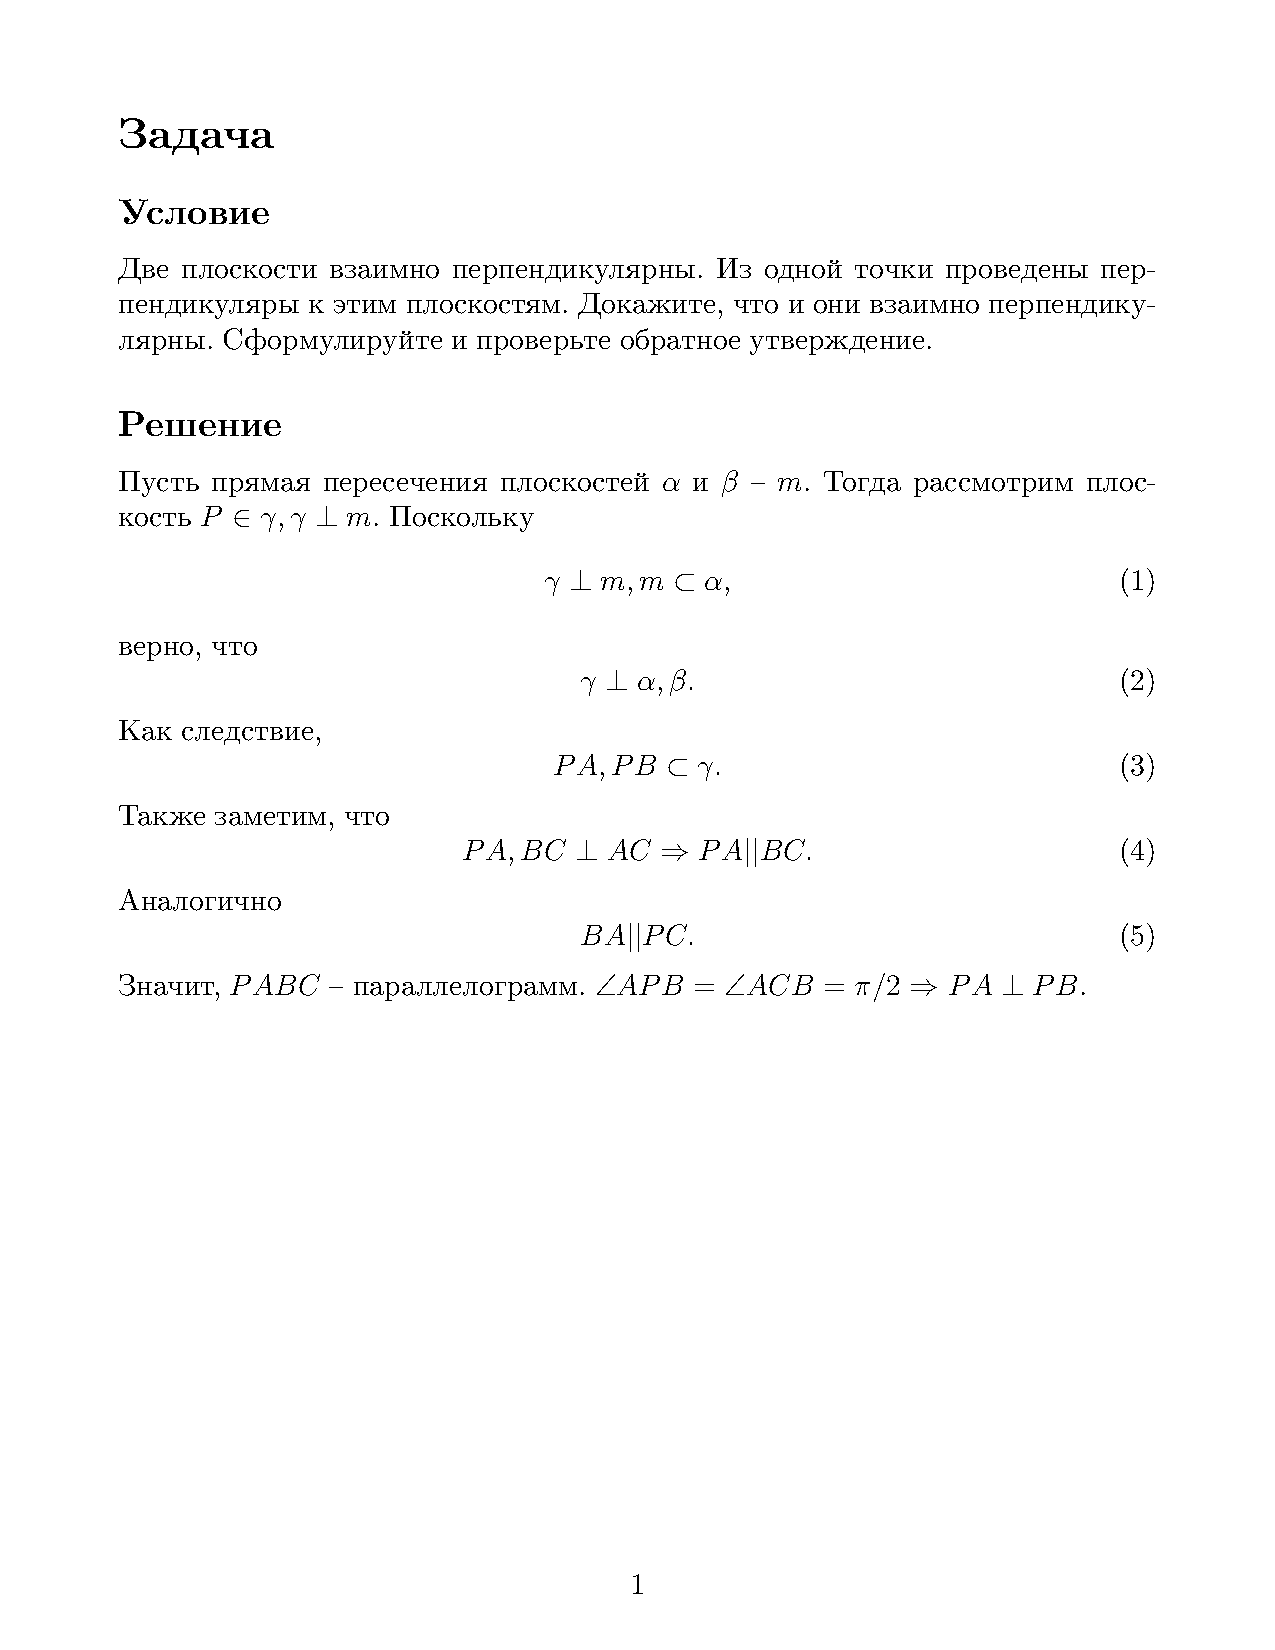
\includegraphics[width=1\textwidth]{{/home/galqiwi/geoma/8.2}.png}
\end{figure}


\end{document}